% !TEX root = presentation.tex
% { % all template changes are local to this group.
%     \begin{frame}[plain]
%         \begin{tikzpicture}[remember picture,overlay]
%             \node[at=(current page.center)] {
%                 \includegraphics[width=\paperwidth]{./img/03_tomb-raider-underworld}
%             };
%         \end{tikzpicture}
%      \end{frame}
% }

\begin{frame}\frametitle{Properties}
	\begin{quote}
		``PN triangles should not deviate too much from the original triangle to preserve the shape and avoid interference with other curved triangles."
		\footnote{\citeauthor{vlachos2001curved}}
	\end{quote}
	\note{\textbf{[Rick]}}
	\note{Stress: important property (of Pn traignle) for a mesh -> else \textbf{gaps} and other \textbf{artifacts} will emerge -> continuity}
\end{frame}

\begin{frame}\frametitle{Continuity}	
	PN triangles have:\footnote{\citeauthor{jiao2005parallel}}
	\begin{itemize}
		\item $C^1$ continuity in the vertex points
		\item $C^0$ continuity along the edges
		\item $C^\infty$ everywhere else
	\end{itemize}
	\note{\textbf{[Rick]}}
	\note[item]{Continuity C0 is important -> no gaps}
	\note[item]{Continuity C0 along edges only when shared normals -> later example of separate normals}
	\note[item]{$C^2$ desirable but not a real problem -> given too us by literature}
\end{frame}

\begin{frame}\frametitle{Sharp Edges}
	\begin{columns}
		\begin{column}[b]{0.22\textwidth}
			\begin{center}
				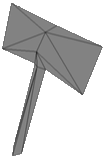
\includegraphics[width=\textwidth]{./img/2_mesh/bluntAxeMesh.png}
				\small{mesh}
			\end{center}	
		\end{column}
		\begin{column}[b]{0.22\textwidth}
			\begin{center}
				
\includegraphics[width=\textwidth]{./img/2_mesh/bluntAxeShaded.png}
				\small{blunt}
			\end{center}	
		\end{column}
		\begin{column}[b]{0.22\textwidth}
			\begin{center}
				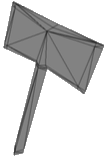
\includegraphics[width=\textwidth]{./img/2_mesh/sharpAxeMesh.png}
				\small{mesh}
			\end{center}	
		\end{column}
		\begin{column}[b]{0.22\textwidth}
			\begin{center}
				
\includegraphics[width=\textwidth]{./img/2_mesh/sharpAxeShaded.png}
				\small{sharp}
			\end{center}	
		\end{column}
	\end{columns}
	\note{\textbf{[Rick]}}
	\note[item]{\textbf{Problem} Pn triangles perform well, but not always desired results.}
	\note[item]{\textbf{Example} Sharp edges.}
	\note[item]{\textbf{Solution} insert more triangles at the sharp edges -> model needs to be changed :(}
\end{frame}	

\begin{frame}\frametitle{Separate Normals}
	\begin{columns}
		\begin{column}{0.4\textwidth}
		\begin{center}
				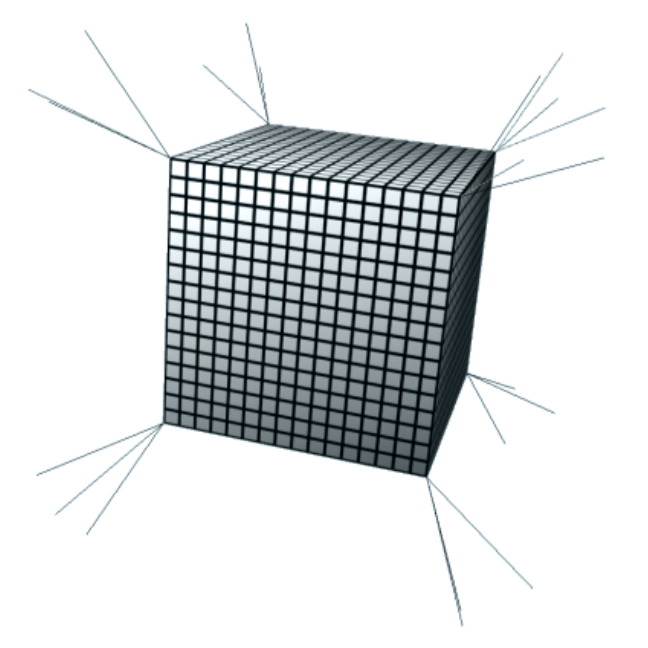
\includegraphics[width=\textwidth]{img/2_mesh/cracksNormals.png}
				\small{normals}
			\end{center}	
		\end{column}
		\begin{column}{0.4\textwidth}
		\begin{center}
				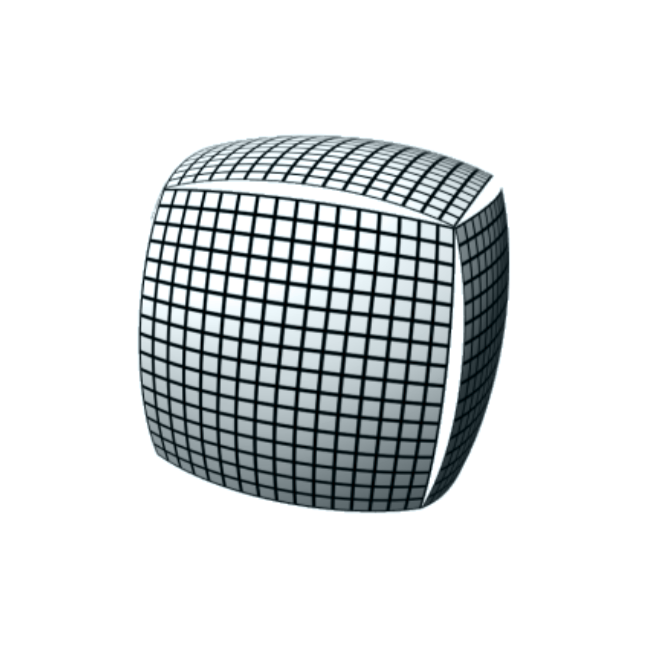
\includegraphics[width=\textwidth]{img/2_mesh/cracks.png}
				\small{cracks}
			\end{center}	
		\end{column}
	\end{columns}
	\note{\textbf{[Rick]}}
	\note[item]{Pn triangle work -> restrict the model -> shared normals}
	\note[item]{Describe slides -> Pn triangle can thus not deal with this}
	\note[item]{Extension exists -> PN-AEN (Adjacent edge normals) (Nvidia)}
\end{frame}
